\section{Statistika}

\subsection{Kvantil}
$\alpha\in [0,1], \alpha - kvantil:$\\
$P(X\leq q_\alpha)=\alpha$\\
$q_\alpha = F_x^{-1}(\alpha)$\\
$q_{\frac{1}{4}}\dots\text{1. kvartil}$\\
$q_{\frac{2}{4}}\dots\text{2. kvartil}\dots \text{mediana}$\\
$q_{\frac{3}{4}}\dots\text{3. kvartil}$\\

\subsection{Kategoricne slucajne spremenljivke}
Za vrednost imajo kategorije.\\
\textbf{Nominalne (imenske)}\\
med kategorijami ni hiearhije:\\
spol: $0=\text{moski}, 1=\text{zenski}$\\
barva las: $1=crna, 2=rjava, 3=rdeca, 4=blondna, 5=bela$\\
\textbf{Ordinalne (urejenostne)}\\
kategorije so urejen, obstaja hiearhija med njimi\\
stopnja bolecine: $0=\text{ni}, 1=\text{blage}, 2=\text{srednje}, 3=\text{mocne}$\\
stopnja izobrazbe: $1=\text{brez}, 2=\text{osnovna sola}, 3=\text{srednja sola}, 4=\text{fakulteta},5=\text{postdiplomski studij}$


\subsection{Nominalna slucajna spremenljivka}
Zabelezili smo krvno skupino nakljucnega vzorca 100 Slovencev.\\
\begin{tabular}{|c | c | c | c | c |}
    \hline
    krvna skupina & 0 & A & B & AB\\
    \hline
    frekvenca f & 38 & 40 & 15 & 7\\
    \hline
\end{tabular}
\begin{center}
    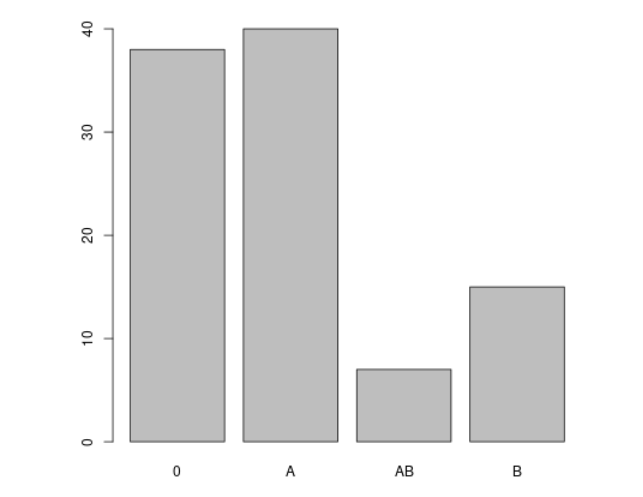
\includegraphics[width=3cm]{barplot.png}    
\end{center}
Lahko ji izracunamo \underline{modus} (najvisji stolpec)
\begin{lstlisting}[language=R]
krv.skupina<-c(rep("O",38),rep("A",40),
rep("B",15), rep("AB",7))
table(krv.skupina)
barplot(table(krv.skupina))
\end{lstlisting}


\subsection{Ordinalna slucajna spremenljivka}
\subsubsection{Opisna statistika}
Podatki se razvrstijo v narascujocem vrstnem redu: $Y_1\leq Y_2\leq \dots Y_n$ (00111122222233).
\begin{itemize}
    \item Modus
    \item Mediana $\displaystyle M_e=\left\{\begin{array}{ll} 
        Y_{(n+1)/2},	&	n-\text{liho}, \\
        \frac{Y_{n/2}+Y_{n/2+1}}{2}, & n-\text{sodo},
    \end{array}\right.$
    \item Kvartili 
    \\ $Q_1$ je mediana prve polovice sortiranih podatkov.
    \\$Q_3$ je mediana druge polovice sortiranih podatkov.
\end{itemize}
\subsubsection{Grafi}
\begin{itemize}
    \item Stolpcni diagram
\end{itemize}


\subsection{Zvezne slucajne spremenljivke}
\subsubsection{Opisna statistika}
\begin{itemize}[leftmargin=*]
    \item \textbf{Vzorcno povprecje} $\overline{X}=\frac{1}{n}\sum\limits_{i=1}^n X_i$\\
    R: $\textbf{mean(teza)}$
    \item \textbf{Popravljeni vzorcni standardni odklon}\\ $S=\sqrt{\frac{1}{n-1}\sum\limits^n_{i=1} (X_i-\overline{X})^2}$\\
    R: $\textbf{sd(teza)}$
    \item \textbf{Povzetek s petimi stevili}\\
    minimum, maksimum, mediana, prvi in tretji kvartil
    R: $\textbf{summary(teza)}$
    
\end{itemize}
\subsubsection{Grafi}
\begin{itemize}[leftmargin=*]
    \item \textbf{Histrogram}
        \begin{itemize}[leftmargin=*]
            \item tezo razdelimo v razrede (intervale) in presetejemo stevilo podatkov v vsakem razredu.
            \item za $n$ podatkov je optimalno \underline{stevilo rezredov}\\$k=\text{ceiling}(\log_2(n))+1$
            \item \underline{dolzina razreda}: $h=\frac{max-min}{k}$
        \end{itemize}

    \item \textbf{Skatla z brki}
        \begin{itemize}[leftmargin=*]
            \item Mediana: navpicna crta v skatli
            \item Meji skatle $Q_1$ in $Q_3$
            \item Dolzina skatle $IQR=Q_3-Q_1$
            \item $\text{Spodnja meja}=Q_1-1.5\cdot\text{IQR}$
            \item $\text{Zgornja meja}=Q_1+1.5\cdot\text{IQR}$
            \item Podatki, ki so manjsi od spodnje ali vecji od zgornje meje se imenujejo osamelci (outliers)

        \end{itemize}
\end{itemize}
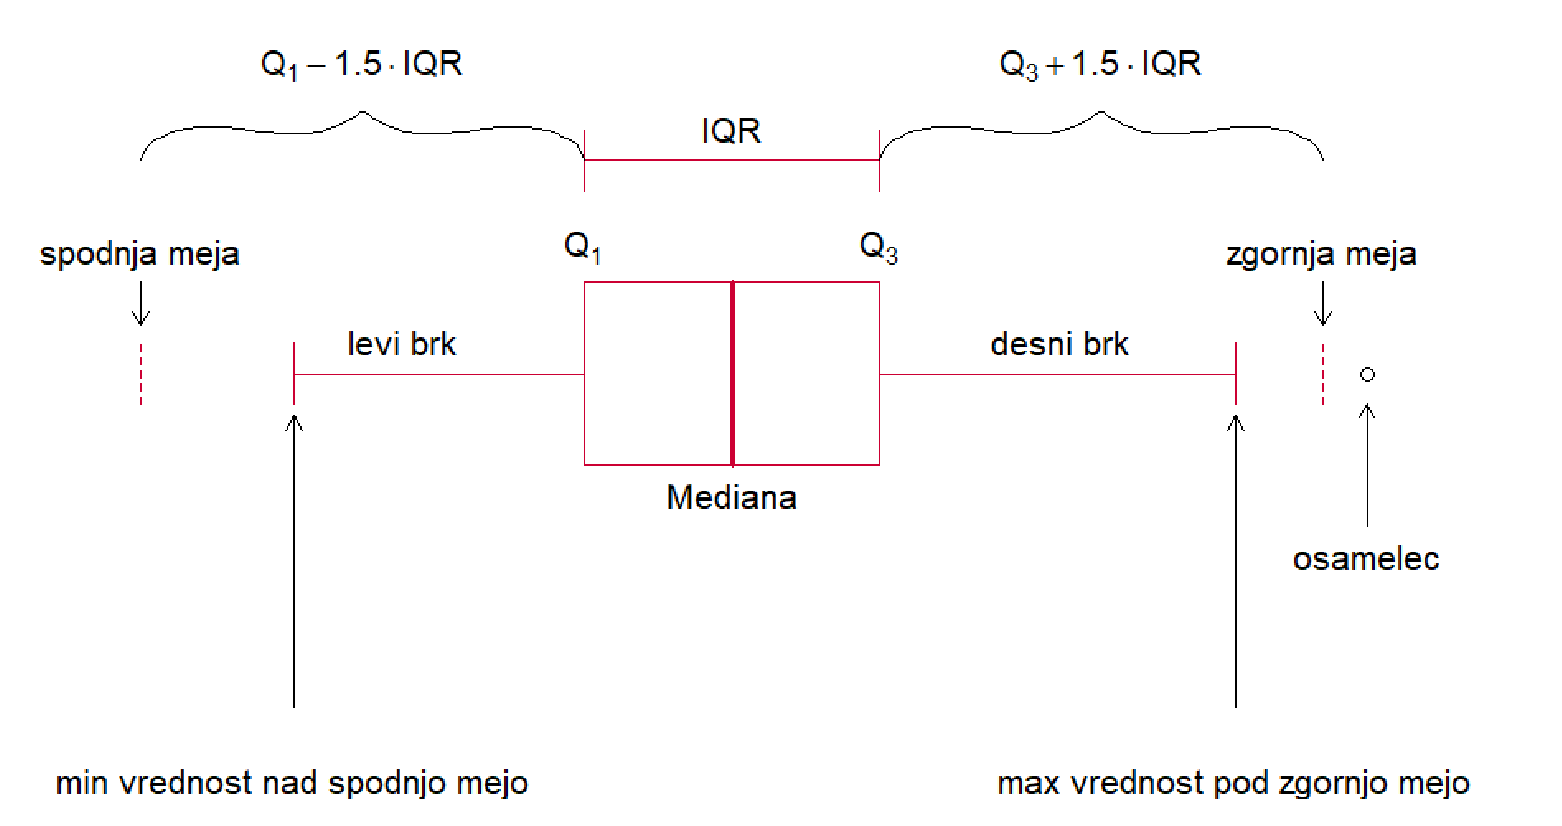
\includegraphics[width=7.5cm]{skatla-z-brki.png}
\subsection{Diskretne slucajne spremelnjivke}
\subsubsection{Opisna statistika}
\begin{itemize}[leftmargin=*]
    \item minimum
    \item maksimum
    \item modus
    \item mediana
    \item kvartili
    \item povprecje
    \item standardni odklon
\end{itemize}
\subsubsection{Grafi}
\begin{itemize}[leftmargin=*]
    \item stolpicni diagram (malo stevilo vrednosti):
    \item histrogram, skatla z brki (vecje stevilo vrednosti):
\end{itemize}

